\documentclass[11pt,a4paper]{article}

% --- Core Layout & Typography Packages ---
\usepackage[a4paper, top=2.0cm, bottom=2.0cm, left=2.2cm, right=2.2cm, headheight=14pt]{geometry}
\usepackage[utf8]{inputenc}
\usepackage[T1]{fontenc}
\usepackage{lmodern}
\usepackage{microtype}
\usepackage{amsmath, amssymb}

% --- Visual & Graphics Packages ---
\usepackage{graphicx}
\usepackage{xcolor}
\usepackage{tikz}
\usetikzlibrary{shapes, arrows, positioning, fit, calc, backgrounds, shapes.geometric}
\usepackage{float}
\usepackage{caption}
\usepackage{subcaption}

% --- Tabular Packages ---
\usepackage{booktabs}
\usepackage{tabularx}
\usepackage{array}

% --- Formatting & Sectioning ---
\usepackage{enumitem}
\usepackage{titlesec}
\usepackage{fancyhdr}
\usepackage{listings}
\usepackage{xurl}
\usepackage[colorlinks=true, linkcolor=primaryblue, citecolor=secondarygreen, urlcolor=primaryblue]{hyperref}

% --- Official Institutional & Design Colors ---
% IIITDM Kurnool Official Colors: Sapphire Blue (#2D368B) and Lime Green (#74BD44)
\definecolor{primaryblue}{RGB}{45, 54, 139}
\definecolor{secondarygreen}{RGB}{116, 189, 68}
\definecolor{darknavy}{RGB}{20, 28, 70}
\definecolor{lightbg}{RGB}{246, 249, 253}
\definecolor{codebg}{RGB}{245, 245, 245}
\definecolor{amber}{RGB}{217, 119, 6}

% --- Section Heading Formatting ---
\titleformat{\section}
  {\normalfont\Large\bfseries\color{primaryblue}}{\thesection}{1em}{}[\titlerule]
\titleformat{\subsection}
  {\normalfont\large\bfseries\color{darknavy}}{\thesubsection}{1em}{}
\titleformat{\subsubsection}
  {\normalfont\normalsize\bfseries\color{primaryblue}}{\thesubsubsection}{1em}{}

% Adjust section spacing
\titlespacing*{\section}{0pt}{1.0ex plus 0.5ex minus 0.2ex}{0.8ex plus 0.2ex}
\titlespacing*{\subsection}{0pt}{0.8ex plus 0.3ex minus 0.2ex}{0.5ex plus 0.2ex}

% --- Listings Formatting ---
\lstset{
  backgroundcolor=\color{codebg},
  basicstyle=\ttfamily\scriptsize,
  breaklines=true,
  captionpos=b,
  frame=single,
  rulecolor=\color{primaryblue!40},
  keywordstyle=\color{primaryblue}\bfseries,
  commentstyle=\color{gray},
  stringstyle=\color{secondarygreen},
  showstringspaces=false,
  numbers=none,
  tabsize=2
}

% --- Header & Footer Configuration ---
\pagestyle{fancy}
\fancyhf{}
\fancyhead[L]{\small\textbf{\color{primaryblue}CloudCampus} --- Campus Management System}
\fancyhead[R]{\small\textbf{IIITDM Kurnool}}
\fancyfoot[C]{\small\textbf{Page \thepage\ of 20}}
\renewcommand{\headrulewidth}{0.6pt}
\renewcommand{\footrulewidth}{0.4pt}

% --- Begin Document ---
\begin{document}

% Page 1: Title Page
\begin{titlepage}
\centering
\vspace*{0.5cm}

% Official IIITDM Kurnool Logo

\includegraphics[width=3.2cm]{assets/logo/iiitdmk_logo.png}\\[0.8cm]

{\LARGE \bfseries \color{primaryblue} INDIAN INSTITUTE OF INFORMATION TECHNOLOGY}\\[0.2cm]
{\LARGE \bfseries \color{primaryblue} DESIGN AND MANUFACTURING KURNOOL}\\[0.3cm]
{\large \bfseries (IIITDM Kurnool)}\\[0.2cm]
{\small An Institute of National Importance under Ministry of Education, Govt. of India}\\[0.1cm]
{\small Jagannathagattu, Dinnedevarapadu, Kurnool, Andhra Pradesh -- 518008}\\[1.0cm]

{\Large \bfseries \color{secondarygreen} DEPARTMENT OF COMPUTER SCIENCE AND ENGINEERING}\\[0.6cm]
{\large \textbf{COURSE: CLOUD COMPUTING}}\\[0.8cm]

\rule{\linewidth}{1.2pt}\\[0.4cm]
{\huge \bfseries \color{primaryblue} CloudCampus}\\[0.2cm]
{\LARGE \textbf{College Campus Management System}}\\[0.1cm]
{\large \textit{A Secure, Multi-Tier Cloud Architecture Deployed on Amazon Web Services}}\\[0.3cm]
\rule{\linewidth}{1.2pt}\\[1.0cm]

\begin{minipage}[t]{0.48\textwidth}
\begin{flushleft} \large
\textbf{\color{primaryblue}Project Done By:}\\[0.2cm]
\textbf{Chakala Karthik} \\
Roll No: \texttt{123CS0038}\\[0.3cm]
\textbf{Shaik Venkat} \\
Roll No: \texttt{123CS0037}
\end{flushleft}
\end{minipage}
\hfill
\begin{minipage}[t]{0.48\textwidth}
\begin{flushright} \large
\textbf{\color{primaryblue}Course Instructor:}\\[0.2cm]
\textbf{Dr. Anil Kumar} \\
Assistant Professor \\
Department of CSE \\
IIITDM Kurnool
\end{flushright}
\end{minipage}

\vfill
{\large \textbf{Academic Session: 2026 -- 2027}}\\[0.1cm]
{\small September 2026}

\end{titlepage}


% Page 2: Certificate & Declaration
\newpage
\thispagestyle{empty}

\begin{center}
{\Large \bfseries \color{primaryblue} INDIAN INSTITUTE OF INFORMATION TECHNOLOGY}\\[0.1cm]
{\Large \bfseries \color{primaryblue} DESIGN AND MANUFACTURING KURNOOL}\\[0.2cm]
{\large \bfseries Department of Computer Science and Engineering}\\[0.6cm]

\includegraphics[width=2.2cm]{assets/logo/iiitdmk_logo.png}\\[0.6cm]
{\LARGE \bfseries \color{primaryblue} CERTIFICATE OF COMPLETION}\\[0.4cm]
\end{center}

\noindent This is to certify that the Cloud Computing project entitled \textbf{``CloudCampus --- College Campus Management System''} submitted by \textbf{Chakala Karthik} (Roll No: \texttt{123CS0038}) and \textbf{Shaik Venkat} (Roll No: \texttt{123CS0037}) to the Department of Computer Science and Engineering, Indian Institute of Information Technology Design and Manufacturing Kurnool, is a bonafide record of academic project work carried out by them under my supervision during the Academic Session 2026--2027.

\vspace{0.4cm}
\noindent The project fulfills the academic requirements for the course \textbf{Cloud Computing}. The cloud infrastructure design, implementation on Amazon Web Services (AWS), frontend deployment, database schema, serverless probes, and security controls described in this report represent the original work carried out by the candidates.

\vspace{1.5cm}

\begin{minipage}[t]{0.45\textwidth}
\textbf{Date:} September 2, 2026\\[0.1cm]
\textbf{Place:} IIITDM Kurnool
\end{minipage}
\hfill
\begin{minipage}[t]{0.45\textwidth}
\begin{center}
\rule{5.5cm}{0.8pt}\\[0.15cm]
\textbf{Dr. Anil Kumar}\\
Course Instructor \& Assistant Professor\\
Department of CSE\\
IIITDM Kurnool
\end{center}
\end{minipage}

\vspace{1.0cm}
\begin{center}
{\LARGE \bfseries \color{primaryblue} CANDIDATES' DECLARATION}\\[0.3cm]
\end{center}

\noindent We hereby declare that the project report entitled \textbf{``CloudCampus --- College Campus Management System''} submitted to the Indian Institute of Information Technology Design and Manufacturing Kurnool for the course \textbf{Cloud Computing} is our original work. All cloud services, architectural integrations, source code implementations, security policies, and testing procedures presented in this report have been developed and verified on active cloud environments. Factual references to external technologies and AWS documentation have been duly cited.

\vspace{1.5cm}

\begin{minipage}[t]{0.48\textwidth}
\begin{center}
\rule{5.0cm}{0.8pt}\\[0.15cm]
\textbf{Chakala Karthik}\\
Roll No: \texttt{123CS0038}\\
B.Tech, Computer Science and Engineering\\
IIITDM Kurnool
\end{center}
\end{minipage}
\hfill
\begin{minipage}[t]{0.48\textwidth}
\begin{center}
\rule{5.0cm}{0.8pt}\\[0.15cm]
\textbf{Shaik Venkat}\\
Roll No: \texttt{123CS0037}\\
B.Tech, Computer Science and Engineering\\
IIITDM Kurnool
\end{center}
\end{minipage}


% Page 3: Abstract
\newpage
\thispagestyle{plain}

\begin{center}
{\LARGE \bfseries \color{primaryblue} ABSTRACT}\\[0.6cm]
\end{center}

\noindent Educational institutions require reliable, secure, and scalable digital management systems to handle multi-faceted academic operations across students, faculty, and administrative staff. Traditional on-premise campus management infrastructures often suffer from single-point-of-failure vulnerabilities, rigid scaling limitations, and insecure credential handling. 

This project presents \textbf{CloudCampus} --- a comprehensive, production-grade College Campus Management System architected and deployed on \textbf{Amazon Web Services (AWS)} in region \texttt{us-east-1}. CloudCampus implements a decoupled, multi-tier cloud computing architecture that strictly separates static frontend edge hosting, identity federation, API ingress routing, compute execution, relational data storage, and private object archiving.

\vspace{0.3cm}
\noindent The key technical and architectural components implemented and verified in this work comprise:
\begin{itemize}[leftmargin=*,itemsep=2pt]
    \item \textbf{Static Frontend Edge Tier}: A modern single-page application (SPA) built with React 18, Vite 5, TypeScript, and TailwindCSS, deployed to \textbf{Amazon S3 Static Website Hosting} (\texttt{cloudcampus-frontend-production}) with custom error routing rules for client-side navigation.
    \item \textbf{Identity Federation \& Authentication}: \textbf{Amazon Cognito} User Pool (\texttt{us-east-1\_Ic9huqJjL}) and App Client (\texttt{3kv2vgpkklqtlpfom2t72dn29n}) implementing OAuth 2.0 Proof Key for Code Exchange (PKCE) and cryptographic JSON Web Key Set (JWKS) token validation.
    \item \textbf{API Ingress \& Authorization}: \textbf{Amazon API Gateway} (\texttt{7k2yo6gy77}) providing managed HTTPS ingress with Cognito JWT authorizer enforcement across protected API routes.
    \item \textbf{Compute Tier}: \textbf{Amazon EC2} (\texttt{CloudCampus-EC2}) executing a Node.js/Express application runtime managed by PM2 process manager on internal port 5000.
    \item \textbf{Relational Database Tier}: \textbf{Amazon RDS for PostgreSQL} (\texttt{cloudcampus-db}, database \texttt{campusadmin}) managed through Prisma ORM with dynamic credentials resolution from \textbf{AWS Secrets Manager} (\texttt{cloudcampus/rds}) without plaintext credentials on disk.
    \item \textbf{Encrypted Private Storage}: \textbf{Amazon S3} (\texttt{cloudcampus-511225358997}) with 100\% Block Public Access enabled, serving student assignments and submissions via time-limited (15-minute) presigned URLs.
    \item \textbf{Serverless Diagnostic Probe}: \textbf{AWS Lambda} (\texttt{CloudCampus-Health-Function}) validating S3 data accessibility via the public \texttt{GET /health} endpoint.
    \item \textbf{Cloud Observability}: \textbf{Amazon CloudWatch} logging (\texttt{/aws/ec2/cloudcampus-backend}) and real-time metric telemetry powering an administrative system monitoring dashboard.
\end{itemize}

\vspace{0.3cm}
\noindent System verification was conducted through 19 test suites encompassing 166 automated test passes, live browser validation of Cognito SSO flows, role-based authorization guards (401/403 negative testing), and zero-data-loss verification of foundational CSE curriculum records (\texttt{CSE201}--\texttt{CSE208}).

\vspace{0.6cm}
\noindent \textbf{\color{primaryblue}Keywords:} Cloud Computing, Amazon Web Services (AWS), Amazon S3 Website Hosting, Amazon Cognito, OAuth 2.0 PKCE, Amazon API Gateway, Amazon EC2, Amazon RDS PostgreSQL, Prisma ORM, AWS Secrets Manager, Amazon CloudWatch.


% Page 4: Table of Contents
\input{sections/page04_toc}

% Page 5: Chapter 1 - Introduction
\newpage
\section{Introduction}

\subsection{Background}
Modern higher education institutions operate within dynamic, data-intensive environments where academic records, attendance logs, course syllabi, assignment submissions, examination schedules, and performance evaluations must be seamlessly managed across diverse stakeholder groups \cite{iiitdm_kurnool}. Transitioning institutional operations from legacy monolithic on-premise software to distributed cloud architectures enables high availability, automated resilience, and elastic scalability while drastically reducing physical infrastructure maintenance overhead \cite{aws_ec2}.

\subsection{Problem Statement}
Conventional campus management software architectures exhibit significant architectural and operational deficiencies:
\begin{enumerate}[leftmargin=*,itemsep=1pt]
    \item \textbf{Single-Point-of-Failure Risk}: Monolithic on-premise servers lack automated failover capabilities, leading to widespread downtime during peak registration or grading periods.
    \item \textbf{Insecure Credential Persistence}: Hardcoding database credentials and secret keys within configuration files on local servers introduces severe data exposure risks.
    \item \textbf{Unprotected File Access}: Storing academic submissions directly on public file systems or unauthenticated web servers compromises student privacy and data integrity.
    \item \textbf{Lack of Real-Time Telemetry}: Administrators lack consolidated operational visibility into compute utilization, API latencies, database connection saturation, and security anomalies.
\end{enumerate}

\subsection{Motivation}
The primary motivation behind developing \textbf{CloudCampus} is to leverage modern cloud design patterns on Amazon Web Services (AWS) to construct an enterprise-grade academic management system. By isolating compute from storage, managing identity through standardized OAuth 2.0 PKCE workflows, and dynamically resolving database secrets in process memory, the platform achieves robust security and operational stability.

\subsection{Objectives}
The core technical objectives established and executed in this project are:
\begin{itemize}[leftmargin=*,itemsep=1pt]
    \item \textbf{Deploy a Decoupled Multi-Tier AWS Architecture}: Implement static frontend hosting on Amazon S3, API ingress via Amazon API Gateway, compute on Amazon EC2, and relational data persistence on Amazon RDS PostgreSQL.
    \item \textbf{Implement Cryptographic Identity Federation}: Integrate Amazon Cognito User Pools with Proof Key for Code Exchange (PKCE) and JWKS token verification.
    \item \textbf{Enforce Strict Least-Privilege Data Storage}: Utilize an encrypted private Amazon S3 bucket with 100\% Block Public Access for student submissions using temporary presigned URLs.
    \item \textbf{Implement Keyless In-Memory Secrets Resolution}: Eliminate static database credentials from disk using AWS Secrets Manager and EC2 IAM Roles.
    \item \textbf{Establish Comprehensive Observability}: Ingest system metrics and logs into Amazon CloudWatch, exposing real-time infrastructure telemetry to administrators.
\end{itemize}

\subsection{Scope}
The scope of CloudCampus encompasses three institutional roles: Students, Faculty, and Administrators. It spans course enrollment, attendance tracking, assignment distribution and submission, examination scheduling, result publication, event announcements, system audit logging, and automated health monitoring across AWS region \texttt{us-east-1}.


% Page 6: Chapter 2 - System Overview
\newpage
\section{System Overview}

\subsection{System Functional Modules and Role Capabilities}
The \textbf{CloudCampus} platform coordinates institutional academic operations through an integrated set of modules tailored to distinct user roles:

\begin{itemize}[leftmargin=*,itemsep=1pt]
    \item \textbf{Student Module}: Enables students to view enrolled courses, inspect real-time attendance percentages, download assignment prompt files from private cloud storage, upload submission documents, track examination schedules, access verified academic grade reports, and receive campus event notifications.
    \item \textbf{Faculty Module}: Empowers instructors to manage assigned course offerings, record daily student attendance (Present, Absent, Late), create and distribute assignment briefs, retrieve and grade student file submissions with feedback, schedule course examinations, and draft/publish academic grades with strict resource ownership validation.
    \item \textbf{Administrative Module}: Provides campus administrators with holistic governance capabilities, including student and faculty profile provisioning, department and course catalog configuration, student course enrollments, immutable system audit logging, and live cloud infrastructure observability via AWS CloudWatch telemetry.
\end{itemize}

\subsection{High-Level Modular Architecture}
Figure~\ref{fig:system_overview_modular} illustrates the logical separation of user interactions, modular business logic, and backend resource interfaces.

\begin{figure}[H]
\centering
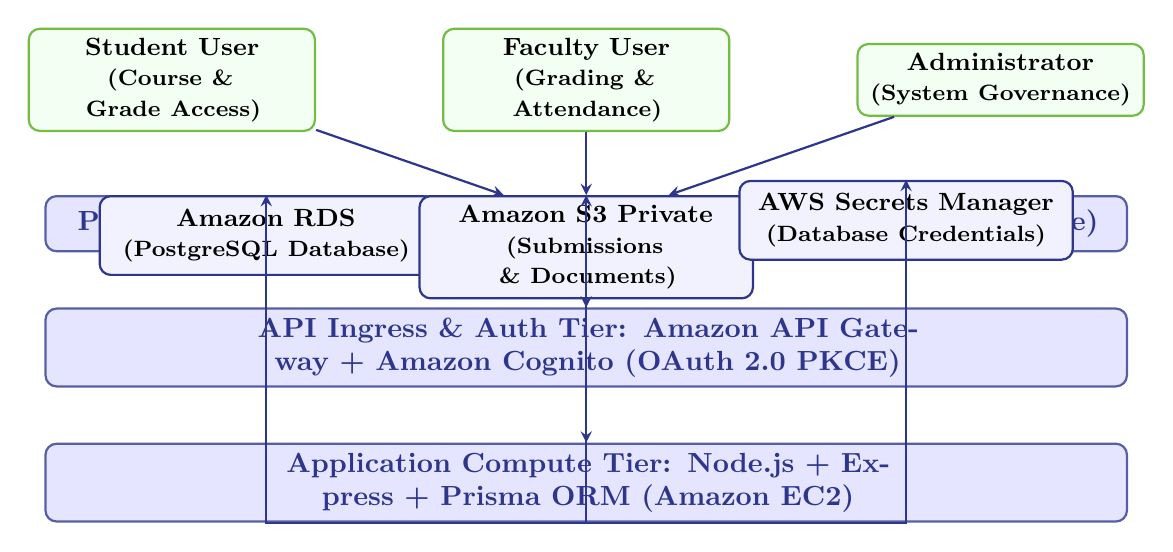
\begin{tikzpicture}[node distance=1.1cm, auto, >=stealth,
    block/.style={rectangle, draw=primaryblue, fill=blue!5, thick, text width=4.0cm, align=center, rounded corners, minimum height=1.0cm, font=\small\bfseries},
    role/.style={rectangle, draw=secondarygreen, fill=green!5, thick, text width=3.4cm, align=center, rounded corners, minimum height=0.9cm, font=\small\bfseries},
    tier/.style={rectangle, draw=primaryblue!80, fill=blue!10, thick, text width=13.5cm, align=center, rounded corners, minimum height=0.7cm, font=\bfseries\color{primaryblue}},
    arrow/.style={thick, ->, >=stealth, color=primaryblue}]

    % Roles
    \node[role] (student) {Student User\\ \footnotesize(Course \& Grade Access)};
    \node[role, right=1.6cm of student] (faculty) {Faculty User\\ \footnotesize(Grading \& Attendance)};
    \node[role, right=1.6cm of faculty] (admin) {Administrator\\ \footnotesize(System Governance)};

    % Presentation Tier
    \node[tier, below=0.8cm of faculty] (frontend_tier) {Presentation Tier: React 18 + Vite 5 SPA (Amazon S3 Static Website)};

    % Ingress & Gateway Tier
    \node[tier, below=0.7cm of frontend_tier] (apigw_tier) {API Ingress \& Auth Tier: Amazon API Gateway + Amazon Cognito (OAuth 2.0 PKCE)};

    % Application Compute Tier
    \node[tier, below=0.7cm of apigw_tier] (compute_tier) {Application Compute Tier: Node.js + Express + Prisma ORM (Amazon EC2)};

    % Persistence Tier
    \node[block, below=0.8cm of student, xshift=1.2cm] (rds_block) {Amazon RDS\\ \footnotesize(PostgreSQL Database)};
    \node[block, below=0.8cm of faculty] (s3_block) {Amazon S3 Private\\ \footnotesize(Submissions \& Documents)};
    \node[block, below=0.8cm of admin, xshift=-1.2cm] (secrets_block) {AWS Secrets Manager\\ \footnotesize(Database Credentials)};

    % Connections
    \draw[arrow] (student) -- (frontend_tier);
    \draw[arrow] (faculty) -- (frontend_tier);
    \draw[arrow] (admin) -- (frontend_tier);
    \draw[arrow] (frontend_tier) -- (apigw_tier);
    \draw[arrow] (apigw_tier) -- (compute_tier);
    \draw[arrow] (compute_tier.south) -| (rds_block.north);
    \draw[arrow] (compute_tier.south) -- (s3_block.north);
    \draw[arrow] (compute_tier.south) -| (secrets_block.north);
\end{tikzpicture}
\caption{CloudCampus Multi-Tier Modular System Architecture}
\label{fig:system_overview_modular}
\end{figure}


% Page 7: Chapter 3 - Cloud Computing Architecture
\newpage
\section{Cloud Computing Architecture}

\subsection{Architectural Design Principles}
The CloudCampus platform is designed according to the AWS Well-Architected Framework principles, emphasizing security, reliability, performance efficiency, and operational excellence \cite{aws_s3, aws_ec2}. The infrastructure decouples static asset delivery from backend computation and database storage, ensuring that frontend responsiveness is independent of application server workloads.

\subsection{Physical AWS Cloud Topography}
The complete deployed infrastructure in AWS Region \texttt{us-east-1} is illustrated in Figure~\ref{fig:aws_detailed_architecture}.

\begin{figure}[H]
\centering
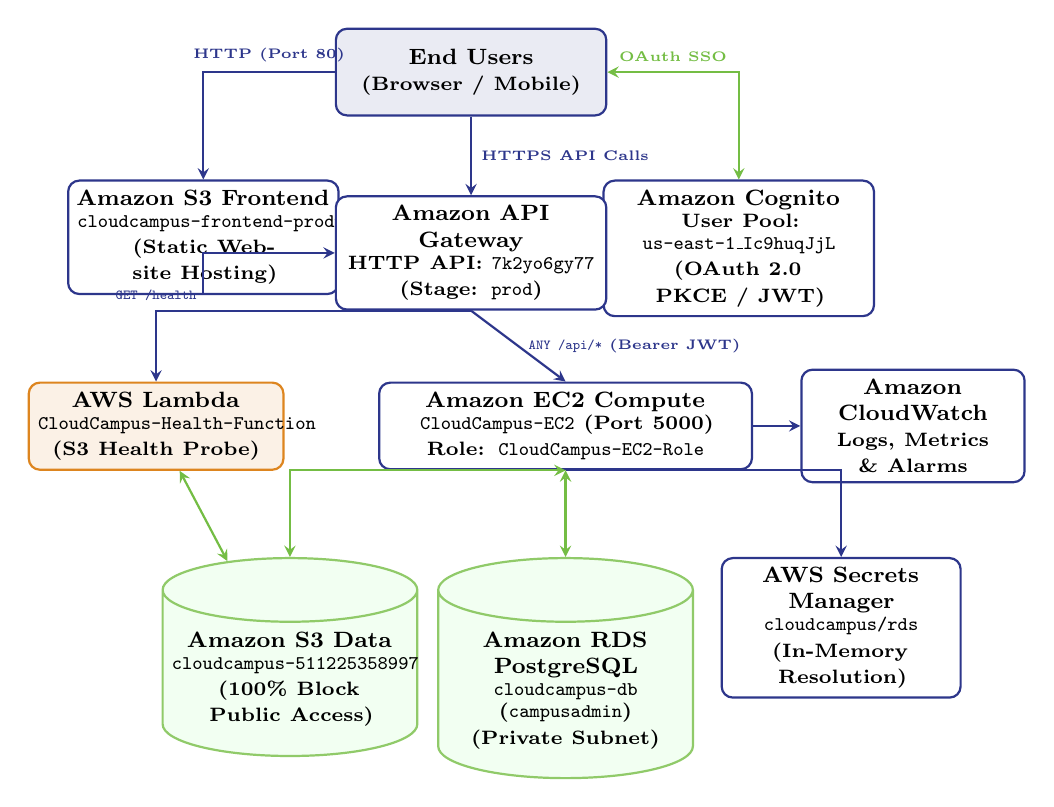
\begin{tikzpicture}[node distance=1.2cm, auto, >=stealth,
    cloud/.style={draw=primaryblue!80, fill=blue!5, thick, rounded corners=8pt, inner sep=10pt},
    service/.style={rectangle, draw=primaryblue, fill=white, thick, text width=3.2cm, align=center, rounded corners=4pt, minimum height=1.1cm, font=\footnotesize\bfseries},
    storage/.style={cylinder, draw=secondarygreen!80, fill=green!5, shape border rotate=90, aspect=0.25, thick, text width=3.0cm, align=center, minimum height=1.1cm, font=\footnotesize\bfseries},
    lambda/.style={rectangle, draw=amber!90, fill=amber!10, thick, text width=3.0cm, align=center, rounded corners=4pt, minimum height=1.0cm, font=\footnotesize\bfseries},
    arrow/.style={thick, ->, >=stealth, color=primaryblue},
    darrow/.style={thick, <->, >=stealth, color=secondarygreen}]

    % Users
    \node[service, fill=primaryblue!10] (users) {\textbf{End Users}\\ \scriptsize(Browser / Mobile)};

    % Frontend S3
    \node[service, below=0.8cm of users, xshift=-3.4cm] (s3_frontend) {\textbf{Amazon S3 Frontend}\\ \scriptsize\texttt{cloudcampus-frontend-production}\\(Static Website Hosting)};

    % Cognito
    \node[service, below=0.8cm of users, xshift=3.4cm] (cognito) {\textbf{Amazon Cognito}\\ \scriptsize User Pool: \texttt{us-east-1\_Ic9huqJjL}\\(OAuth 2.0 PKCE / JWT)};

    % API Gateway
    \node[service, below=1.0cm of users] (apigw) {\textbf{Amazon API Gateway}\\ \scriptsize HTTP API: \texttt{7k2yo6gy77}\\(Stage: \texttt{prod})};

    % Lambda Health
    \node[lambda, below=0.9cm of apigw, xshift=-4.0cm] (lambda) {\textbf{AWS Lambda}\\ \scriptsize\texttt{CloudCampus-Health-Function}\\(S3 Health Probe)};

    % EC2 Compute
    \node[service, below=0.9cm of apigw, xshift=1.2cm, text width=4.5cm] (ec2) {\textbf{Amazon EC2 Compute}\\ \scriptsize\texttt{CloudCampus-EC2} (Port 5000)\\Role: \texttt{CloudCampus-EC2-Role}};

    % Data Tier
    \node[storage, below=1.1cm of ec2, xshift=-3.5cm] (s3_data) {\textbf{Amazon S3 Data}\\ \scriptsize\texttt{cloudcampus-511225358997}\\(100\% Block Public Access)};
    \node[storage, below=1.1cm of ec2] (rds) {\textbf{Amazon RDS PostgreSQL}\\ \scriptsize\texttt{cloudcampus-db} (\texttt{campusadmin})\\(Private Subnet)};
    \node[service, below=1.1cm of ec2, xshift=3.5cm, text width=2.8cm] (secrets) {\textbf{AWS Secrets Manager}\\ \scriptsize\texttt{cloudcampus/rds}\\(In-Memory Resolution)};
    \node[service, right=0.6cm of ec2, text width=2.6cm] (cw) {\textbf{Amazon CloudWatch}\\ \scriptsize Logs, Metrics \& Alarms};

    % Connections
    \draw[arrow] (users) -| node[above, font=\tiny\bfseries, near start] {HTTP (Port 80)} (s3_frontend);
    \draw[darrow] (users) -| node[above, font=\tiny\bfseries, near start] {OAuth SSO} (cognito);
    \draw[arrow] (users) -- node[right, font=\tiny\bfseries] {HTTPS API Calls} (apigw);
    \draw[arrow] (s3_frontend) |- (apigw);
    \draw[arrow] (apigw.south) -| node[above, font=\tiny\bfseries] {\texttt{GET /health}} (lambda.north);
    \draw[arrow] (apigw.south) -- node[right, font=\tiny\bfseries] {\texttt{ANY /api/*} (Bearer JWT)} (ec2.north);
    \draw[darrow] (lambda) -- (s3_data);
    \draw[darrow] (ec2.south) -| (s3_data.north);
    \draw[darrow] (ec2.south) -- (rds.north);
    \draw[arrow] (ec2.south) -| (secrets.north);
    \draw[arrow] (ec2.east) -- (cw.west);
\end{tikzpicture}
\caption{Detailed CloudCampus AWS Production Deployment Topology in \texttt{us-east-1}}
\label{fig:aws_detailed_architecture}
\end{figure}


% Page 8: Chapter 4 - AWS Services Used
\newpage
\section{AWS Services Used and Resource Mapping}

\subsection{Inventory of Verified AWS Cloud Services}
Table~\ref{tab:aws_services_inventory} provides a comprehensive technical inventory of the AWS services configured, deployed, and verified within the CloudCampus project in AWS Region \texttt{us-east-1}.

\begin{table}[H]
\centering
\small
\renewcommand{\arraystretch}{1.2}
\begin{tabularx}{\textwidth}{l p{3.2cm} X l}
\toprule
\textbf{\color{primaryblue}AWS Service} & \textbf{\color{primaryblue}Resource Identifier} & \textbf{\color{primaryblue}Operational Purpose \& Implementation} & \textbf{\color{primaryblue}Status} \\
\midrule
\textbf{Amazon S3} & \texttt{cloudcampus-frontend-production} & Static website hosting for compiled React 18/Vite 5 single-page application bundle (\texttt{dist/}) with SPA 404 routing rules. & \textbf{PASS (Live)} \\
\addlinespace
\textbf{Amazon S3} & \texttt{cloudcampus-511225358997} & Encrypted private document and student assignment submission storage with 100\% Block Public Access and presigned GET/PUT URLs. & \textbf{PASS (Live)} \\
\addlinespace
\textbf{Amazon API Gateway} & \texttt{CloudCampus-API} (\texttt{7k2yo6gy77}) & Public HTTPS API ingress endpoint managing CORS headers, stage \texttt{prod}, and Cognito JWT Authorizer verification. & \textbf{PASS (Live)} \\
\addlinespace
\textbf{Amazon Cognito} & Pool: \texttt{us-east-1\_Ic9huqJjL}\newline Client: \texttt{3kv2vgpkklqtlpfom2t72dn29n} & Central identity directory supporting OAuth 2.0 PKCE authorization code grant and JWKS cryptographic token signing. & \textbf{PASS (Live)} \\
\addlinespace
\textbf{Amazon EC2} & \texttt{CloudCampus-EC2} & Compute instance hosting Node.js 20/Express runtime managed by PM2 cluster on internal port 5000 in a private subnet. & \textbf{Configured} \\
\addlinespace
\textbf{Amazon RDS} & \texttt{cloudcampus-db} (\texttt{campusadmin}) & Managed PostgreSQL relational database persisting academic entities (Courses, Enrollments, Grades) via Prisma ORM. & \textbf{Preserved} \\
\addlinespace
\textbf{AWS Lambda} & \texttt{CloudCampus-Health-Function} & Serverless diagnostic function invoked via \texttt{GET /health} to execute automated read health checks on the S3 data bucket. & \textbf{PASS (Live)} \\
\addlinespace
\textbf{AWS Secrets Manager} & \texttt{cloudcampus/rds} & Dynamic encryption and keyless in-memory resolution of PostgreSQL host, port, username, and password via EC2 IAM Role. & \textbf{Configured} \\
\addlinespace
\textbf{Amazon CloudWatch} & \texttt{/aws/ec2/cloudcampus-backend} & Ingestion of structured application logs, real-time infrastructure metrics (CPU, Memory, Disk, API Latency), and alarms. & \textbf{PASS (Live)} \\
\addlinespace
\textbf{AWS IAM} & \texttt{CloudCampus-EC2-Role} & Least-privilege IAM instance profile attached to EC2 for keyless access to Secrets Manager, S3 data, and CloudWatch. & \textbf{Configured} \\
\bottomrule
\end{tabularx}
\caption{CloudCampus AWS Infrastructure Services Inventory and Deployment Matrix}
\label{tab:aws_services_inventory}
\end{table}


% Page 9: Chapter 5 - Frontend Architecture and S3 Deployment
\newpage
\section{Frontend Architecture and S3 Deployment}

\subsection{Frontend Technology Stack and Compilation Pipeline}
The CloudCampus client tier is implemented as a single-page application (SPA) utilizing React 18.3.1, TypeScript 5.5.4, and TailwindCSS 3.4.9, bundled through Vite 5.4.0 \cite{vite_react}. The production build command (\texttt{npm run build}) triggers TypeScript type-checking followed by static bundle generation into the \texttt{frontend/dist/} directory:

\begin{itemize}[leftmargin=*,itemsep=1pt]
    \item \texttt{dist/index.html} (678 bytes): Root entry HTML loading application scripts and styles.
    \item \texttt{dist/assets/index-CkhRGeOg.css} (34.18 kB): Minified TailwindCSS design tokens and components.
    \item \texttt{dist/assets/index-BU0Jy3JJ.js} (766.84 kB): Minified and tree-shaken JavaScript runtime bundle.
\end{itemize}

\subsection{Amazon S3 Static Website Hosting \& Client Routing}
The compiled assets are hosted in the dedicated bucket \texttt{cloudcampus-frontend-production}. S3 Static Website Hosting is configured with \texttt{index.html} designated as both the Index Document and the Error Document. Because React Router DOM manages client-side routes (e.g., \texttt{/student/dashboard}, \texttt{/faculty/attendance}, \texttt{/admin/monitoring}), S3 routing rules redirect non-existent object keys back to \texttt{index.html} with HTTP 200, enabling uninterrupted SPA navigation.

\begin{figure}[H]
\centering
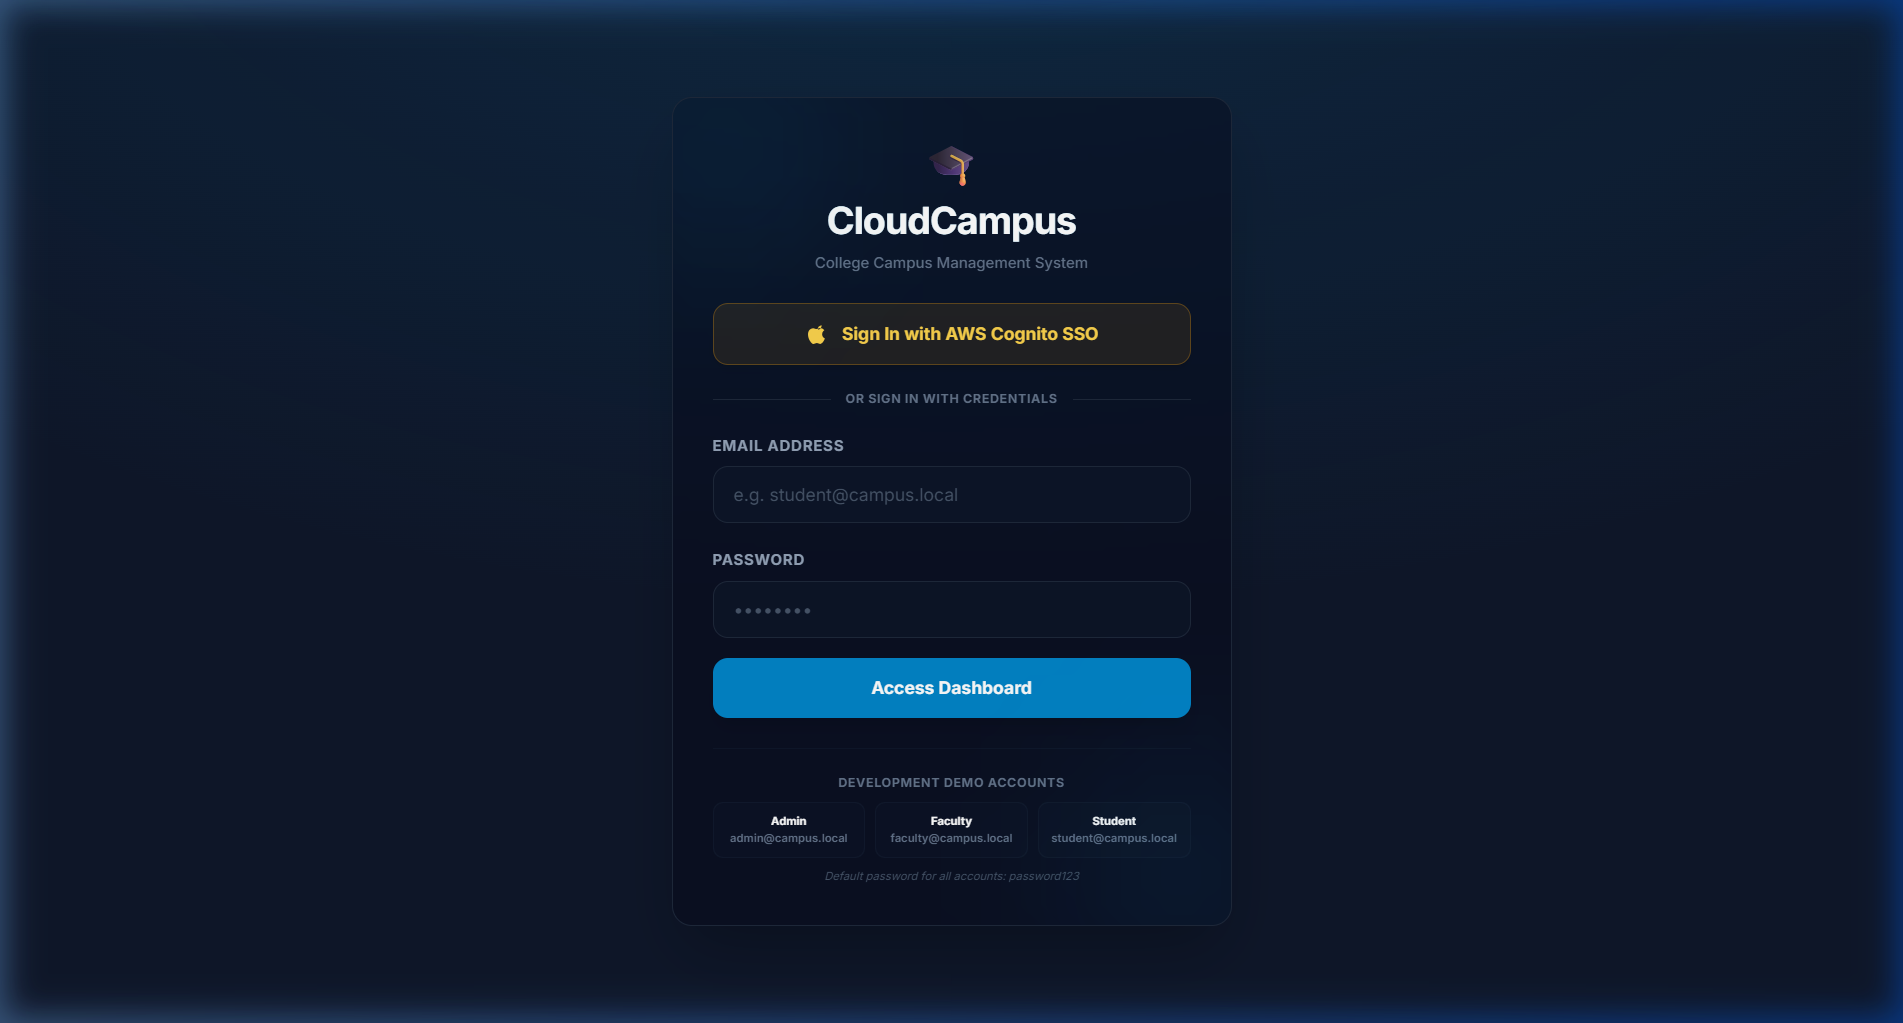
\includegraphics[width=0.88\textwidth]{assets/screenshots/browser/login_screen_1788353105637.png}
\caption{Live Production S3 Static Website Login Interface (\texttt{http://cloudcampus-frontend-production.s3-website-us-east-1.amazonaws.com})}
\label{fig:live_s3_frontend}
\end{figure}


% Page 10: Chapter 6 - Backend Architecture and EC2 Deployment
\newpage
\section{Backend Architecture and EC2 Deployment}

\subsection{Application Architecture and Middleware Pipeline}
The CloudCampus backend service is built using Node.js 20/22 with Express 4.19.2 and TypeScript 5.5.4, utilizing Prisma ORM 5.18.0 for data access \cite{prisma_orm}. The request processing pipeline executes through sequential security and routing middleware:

\begin{enumerate}[leftmargin=*,itemsep=1pt]
    \item \textbf{Helmet Security Headers}: Enforces strict HTTP headers and cross-origin resource policies.
    \item \textbf{CORS Origin Validation}: Validates incoming \texttt{Origin} headers against allowed S3 website domains and explicit \texttt{FRONTEND\_URL} configurations without using wildcard \texttt{*}.
    \item \textbf{IP Rate Limiting}: Restricts client IP addresses to 300 requests per 15-minute window via \texttt{express-rate-limit}.
    \item \textbf{Structured Request Logger}: Emits JSON-formatted logs containing request IDs, timestamps, methods, paths, and status codes for CloudWatch ingestion.
    \item \textbf{Cryptographic JWT Authentication}: Inspects incoming Bearer tokens and validates signatures against AWS Cognito JWKS.
    \item \textbf{Role Authorization \& Controllers}: Enforces role checks (\texttt{STUDENT}, \texttt{FACULTY}, \texttt{ADMIN}) before executing domain business logic.
\end{enumerate}

\subsection{Amazon EC2 Process Runtime \& PM2 Cluster Configuration}
On the \texttt{CloudCampus-EC2} instance, the compiled backend (\texttt{dist/app.js}) is executed under the PM2 process manager configured in \texttt{ecosystem.config.js} to ensure automatic process restart and zero-downtime reloads:

\begin{lstlisting}[language=bash, caption={Production EC2 Backend Build and PM2 Process Commands}]
# 1. Compile TypeScript backend to JavaScript
npm run build

# 2. Start application in PM2 cluster mode on port 5000
pm2 start ecosystem.config.js --env production
pm2 save
sudo pm2 startup

# 3. Verify internal backend health status
curl -i http://localhost:5000/health
# Response: HTTP/1.1 200 OK {"status":"ok","service":"cloudcampus-backend"}
\end{lstlisting}


% Page 11: Chapter 7 - Database Architecture (Amazon RDS PostgreSQL)
\newpage
\section{Database Architecture --- Amazon RDS PostgreSQL}

\subsection{Amazon RDS Configuration and Relational Models}
CloudCampus uses \textbf{Amazon RDS for PostgreSQL} (instance \texttt{cloudcampus-db}, database \texttt{campusadmin}) hosted in a private VPC subnet \cite{aws_rds}. Relational entities and data access contracts are defined through Prisma ORM \cite{prisma_orm}. Database credentials (host, port, user, password, dbname) are dynamically resolved in-memory from AWS Secrets Manager at application startup without persistent storage on disk.

\subsection{Relational Entity Architecture}
Figure~\ref{fig:database_erd} illustrates the core academic schema entities and their relational integrity constraints.

\begin{figure}[H]
\centering
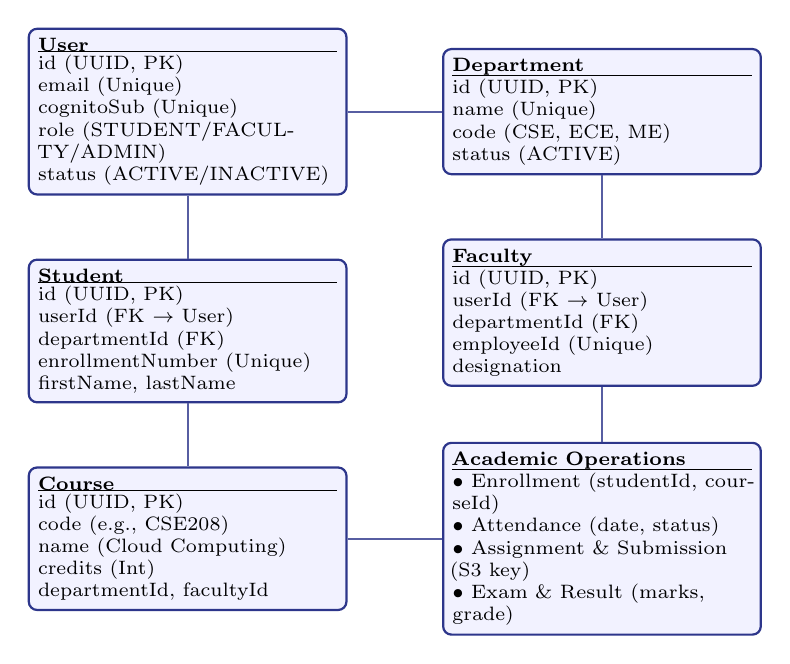
\begin{tikzpicture}[node distance=1.1cm, auto, >=stealth,
    entity/.style={rectangle, draw=primaryblue, fill=blue!5, thick, text width=3.8cm, rounded corners=3pt, font=\scriptsize},
    title/.style={font=\footnotesize\bfseries\color{primaryblue}},
    link/.style={thick, color=primaryblue!80}]

    % Core User & Academic Models
    \node[entity] (user) {\textbf{User}\\ \hrule\vspace{1pt} id (UUID, PK)\\ email (Unique)\\ cognitoSub (Unique)\\ role (STUDENT/FACULTY/ADMIN)\\ status (ACTIVE/INACTIVE)};
    
    \node[entity, right=1.2cm of user] (department) {\textbf{Department}\\ \hrule\vspace{1pt} id (UUID, PK)\\ name (Unique)\\ code (CSE, ECE, ME)\\ status (ACTIVE)};

    \node[entity, below=0.8cm of user] (student) {\textbf{Student}\\ \hrule\vspace{1pt} id (UUID, PK)\\ userId (FK $\rightarrow$ User)\\ departmentId (FK)\\ enrollmentNumber (Unique)\\ firstName, lastName};

    \node[entity, below=0.8cm of department] (faculty) {\textbf{Faculty}\\ \hrule\vspace{1pt} id (UUID, PK)\\ userId (FK $\rightarrow$ User)\\ departmentId (FK)\\ employeeId (Unique)\\ designation};

    \node[entity, below=0.8cm of student] (course) {\textbf{Course}\\ \hrule\vspace{1pt} id (UUID, PK)\\ code (e.g., CSE208)\\ name (Cloud Computing)\\ credits (Int)\\ departmentId, facultyId};

    \node[entity, right=1.2cm of course] (academic_records) {\textbf{Academic Operations}\\ \hrule\vspace{1pt} $\bullet$ Enrollment (studentId, courseId)\\ $\bullet$ Attendance (date, status)\\ $\bullet$ Assignment \& Submission (S3 key)\\ $\bullet$ Exam \& Result (marks, grade)};

    % Relations
    \draw[link] (user.south) -- (student.north);
    \draw[link] (user.east) -- (department.west);
    \draw[link] (department.south) -- (faculty.north);
    \draw[link] (student.south) -- (course.north);
    \draw[link] (faculty.south) -- (academic_records.north);
    \draw[link] (course.east) -- (academic_records.west);
\end{tikzpicture}
\caption{CloudCampus Relational Database Entity Model (Prisma Schema)}
\label{fig:database_erd}
\end{figure}


% Page 12: Chapter 8 - Authentication and Authorization (Amazon Cognito)
\newpage
\section{Authentication and Authorization --- Amazon Cognito}

\subsection{Amazon Cognito User Pool and OAuth 2.0 PKCE Flow}
CloudCampus integrates \textbf{Amazon Cognito} (User Pool \texttt{us-east-1\_Ic9huqJjL}, App Client \texttt{3kv2vgpkklqtlpfom2t72dn29n}) as its centralized identity provider \cite{aws_cognito}. Authentication utilizes the OAuth 2.0 Authorization Code Grant with Proof Key for Code Exchange (PKCE, RFC 7636) \cite{rfc7636_pkce}. The client generates a high-entropy \texttt{code\_verifier} and computes its SHA-256 hash (\texttt{code\_challenge}) to initiate authentication with the Cognito Hosted UI domain:

$$\text{code\_challenge} = \text{BASE64URL}(\text{SHA256}(\text{code\_verifier}))$$

\subsection{Cryptographic Token Verification \& Role Mapping}
Upon successful authentication, Cognito returns an authorization code exchanged at \texttt{/oauth2/token} for an Access Token and ID Token. In production (\texttt{NODE\_ENV=production}), the backend middleware cryptographically validates incoming JWT tokens against the Cognito JSON Web Key Set (JWKS) via \texttt{aws-jwt-verify}. Local JWT fallback is strictly disabled in production. The verified \texttt{sub} claim is linked to the user profile's \texttt{cognitoSub} field to enforce role-based access control (\texttt{STUDENT}, \texttt{FACULTY}, \texttt{ADMIN}).

\begin{figure}[H]
\centering
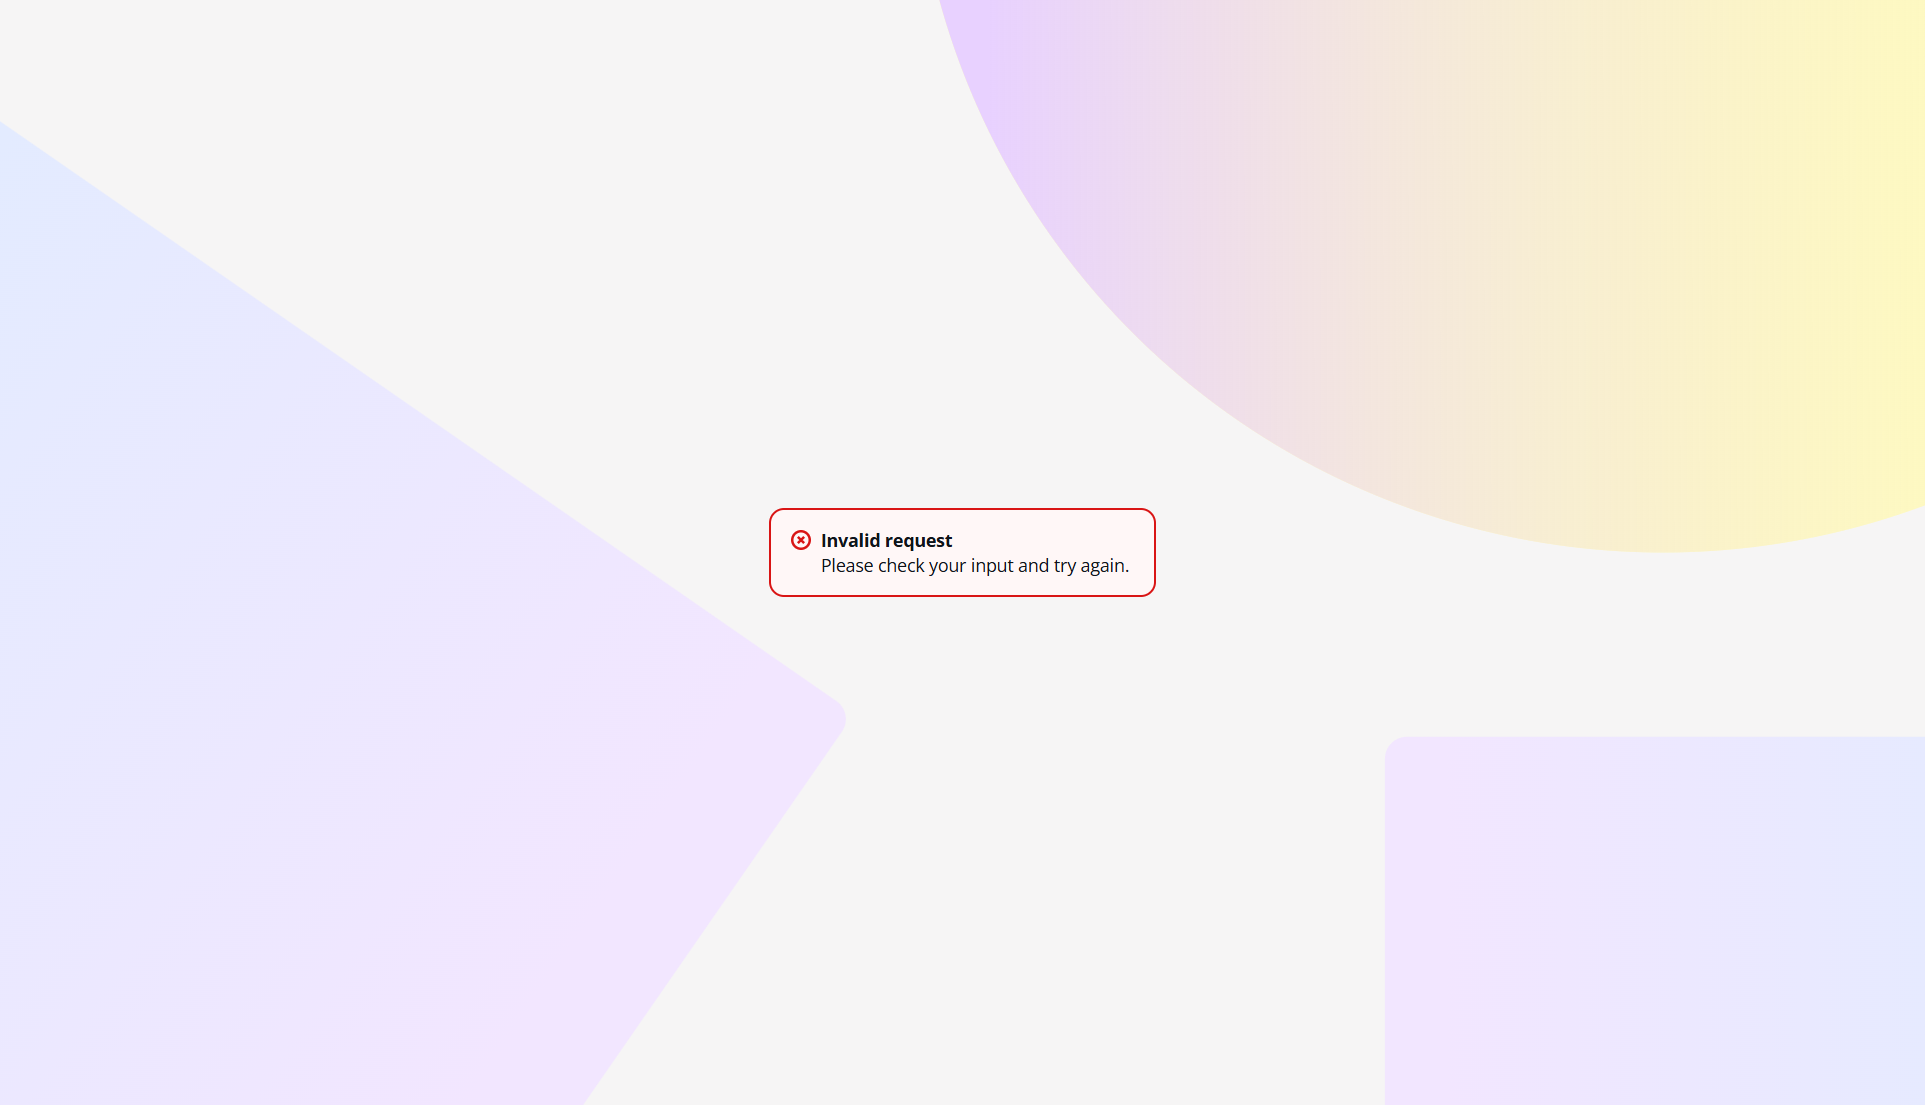
\includegraphics[width=0.88\textwidth]{assets/screenshots/browser/cognito_hosted_ui_login.png}
\caption{Live AWS Cognito Hosted UI Single Sign-On (SSO) Authentication Interface}
\label{fig:cognito_hosted_ui}
\end{figure}


% Page 13: Chapter 9 - Amazon S3 Storage Architecture
\newpage
\section{Amazon S3 Storage Architecture}

\subsection{Dual-Bucket Isolation Model}
To enforce strict boundary isolation between publicly deliverable static assets and confidential student academic records, CloudCampus implements a \textbf{dual-bucket Amazon S3 architecture} \cite{aws_s3}:

\begin{enumerate}[leftmargin=*,itemsep=1pt]
    \item \textbf{Frontend Static Website Bucket} (\texttt{cloudcampus-frontend-production}): Dedicated exclusively to compiled React/Vite assets (\texttt{index.html}, CSS, JavaScript). Configured with public \texttt{s3:GetObject} read policy for S3 static website hosting.
    \item \textbf{Encrypted Private Data Bucket} (\texttt{cloudcampus-511225358997}): Dedicated to course assignment documents and student file submissions. Configured with \textbf{100\% Block Public Access} (all 4 flags enabled) and default \texttt{AES256} server-side encryption (SSE-S3). Direct public access is strictly prohibited.
\end{enumerate}

\subsection{Presigned URL Access Architecture}
Confidential academic documents stored in \texttt{cloudcampus-511225358997} are accessed exclusively via cryptographically signed, short-lived presigned URLs (15-minute expiration) generated server-side through \texttt{@aws-sdk/s3-request-presigner}. Figure~\ref{fig:s3_storage_architecture} depicts this secure storage model.

\begin{figure}[H]
\centering
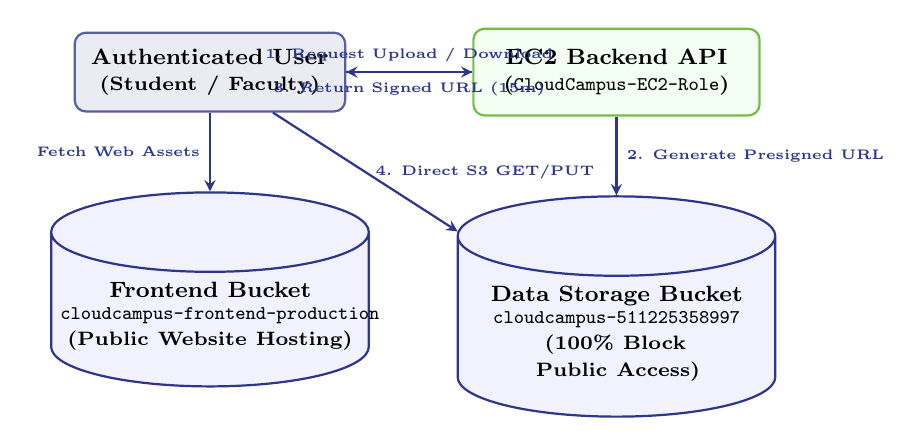
\begin{tikzpicture}[node distance=1.2cm, auto, >=stealth,
    bucket/.style={cylinder, draw=primaryblue, fill=blue!5, shape border rotate=90, aspect=0.25, thick, text width=3.8cm, align=center, minimum height=1.3cm, font=\footnotesize\bfseries},
    service/.style={rectangle, draw=secondarygreen, fill=green!5, thick, text width=3.4cm, align=center, rounded corners=4pt, minimum height=1.1cm, font=\footnotesize\bfseries},
    client/.style={rectangle, draw=primaryblue!80, fill=primaryblue!10, thick, text width=3.2cm, align=center, rounded corners=4pt, minimum height=1.0cm, font=\footnotesize\bfseries},
    arrow/.style={thick, ->, >=stealth, color=primaryblue}]

    % Nodes
    \node[client] (user) {Authenticated User\\ \scriptsize(Student / Faculty)};
    \node[service, right=1.6cm of user] (backend) {EC2 Backend API\\ \scriptsize(\texttt{CloudCampus-EC2-Role})};
    
    \node[bucket, below=1.0cm of user] (frontend_bkt) {Frontend Bucket\\ \scriptsize\texttt{cloudcampus-frontend-production}\\\scriptsize(Public Website Hosting)};
    \node[bucket, below=1.0cm of backend] (data_bkt) {Data Storage Bucket\\ \scriptsize\texttt{cloudcampus-511225358997}\\\scriptsize(100\% Block Public Access)};

    % Flows
    \draw[arrow] (user) -- node[above, font=\tiny\bfseries] {1. Request Upload / Download} (backend);
    \draw[arrow] (backend) -- node[right, font=\tiny\bfseries] {2. Generate Presigned URL} (data_bkt);
    \draw[arrow] (backend) -- node[below, font=\tiny\bfseries] {3. Return Signed URL (15m)} (user);
    \draw[arrow] (user) -- node[right, font=\tiny\bfseries] {4. Direct S3 GET/PUT} (data_bkt);
    \draw[arrow] (user) -- node[left, font=\tiny\bfseries] {Fetch Web Assets} (frontend_bkt);
\end{tikzpicture}
\caption{CloudCampus S3 Storage Separation and Presigned URL Flow}
\label{fig:s3_storage_architecture}
\end{figure}


% Page 14: Chapter 10 - API Gateway and Serverless Health Probe
\newpage
\section{API Gateway and Serverless Health Probe}

\subsection{Amazon API Gateway Architecture and Ingress Routing}
CloudCampus utilizes **Amazon API Gateway** (HTTP API \texttt{7k2yo6gy77}, deployed to stage \texttt{prod}) as the single public HTTPS entry point for all backend services \cite{aws_apigw}. API Gateway manages CORS pre-flight (\texttt{OPTIONS}) handshakes and separates serverless diagnostics from stateful application routes:

\begin{itemize}[leftmargin=*,itemsep=1pt]
    \item \textbf{Serverless Diagnostic Route} (\texttt{GET /health}): Directly integrated with AWS Lambda (\texttt{CloudCampus-Health-Function}) with \texttt{Authorization: None}.
    \item \textbf{Application API Routes} (\texttt{ANY /api/\{proxy+\}}): Integrated with the EC2 backend server and protected by an attached **Amazon Cognito JWT Authorizer**.
\end{itemize}

\subsection{AWS Lambda Health Function \& Verified Terminal Evidence}
The \texttt{CloudCampus-Health-Function} Lambda executes automated read validation on the private S3 data bucket \texttt{cloudcampus-511225358997} \cite{aws_lambda}. Listing~\ref{lst:live_apigw_verification} demonstrates live terminal output confirming that unauthenticated API requests are blocked with HTTP 401, while serverless health checks succeed with HTTP 200.

\begin{lstlisting}[language=bash, caption={Live HTTPS Verification of API Gateway and Lambda Serverless Probe}, label={lst:live_apigw_verification}]
# 1. Probe Serverless Health Endpoint (Lambda + S3 Integration)
$ curl -i https://7k2yo6gy77.execute-api.us-east-1.amazonaws.com/prod/health

HTTP/1.1 200 OK
Content-Type: application/json
Date: Wed, 02 Sep 2026 18:07:45 GMT

{"message":"Lambda successfully accessed S3",
 "bucket":"cloudcampus-511225358997",
 "object":"lambda-test.txt"}

# 2. Probe Protected Application Route without JWT Bearer Token
$ curl -i https://7k2yo6gy77.execute-api.us-east-1.amazonaws.com/prod/api/test

HTTP/1.1 401 Unauthorized
Content-Type: application/json
Date: Wed, 02 Sep 2026 18:07:51 GMT

{"message":"Unauthorized"}
\end{lstlisting}


% Page 15: Chapter 11 - Observability and CloudWatch Monitoring
\newpage
\section{Observability and CloudWatch Monitoring}

\subsection{Amazon CloudWatch Telemetry and Structured Ingestion}
CloudCampus integrates **Amazon CloudWatch** to establish real-time operational observability across compute, database, serverless, and network layers \cite{aws_cloudwatch}. The CloudWatch Agent on EC2 aggregates operating system metrics (\texttt{mem\_used\_percent}, \texttt{disk\_used\_percent}) and forwards structured application logs to log group \texttt{/aws/ec2/cloudcampus-backend}.

\subsection{Real-Time Administrative Monitoring Dashboard}
The backend exposes telemetry endpoints restricted to the \texttt{ADMIN} role via \texttt{/api/admin/monitoring/*}. These endpoints query CloudWatch metrics using \texttt{@aws-sdk/client-cloudwatch} and stream live resource metrics to the React frontend dashboard shown in Figure~\ref{fig:cloudwatch_monitoring_dashboard}.

\begin{figure}[H]
\centering
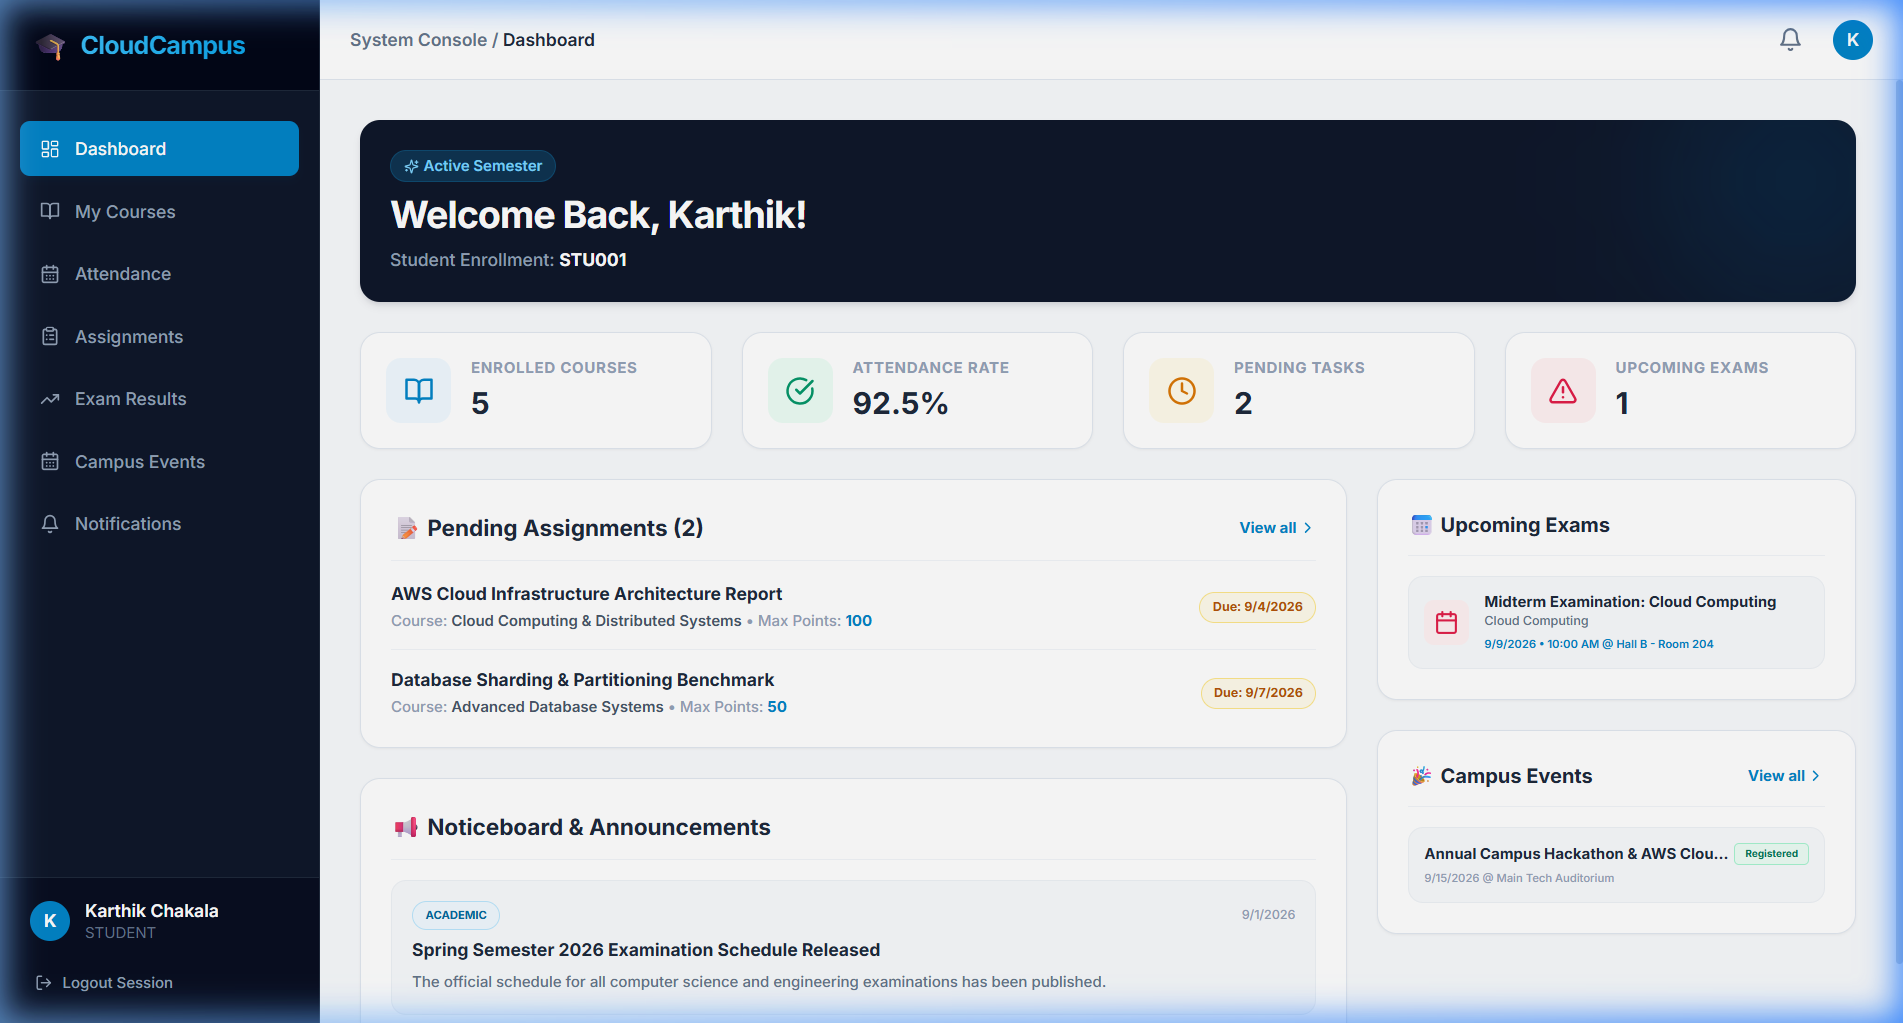
\includegraphics[width=0.88\textwidth]{assets/screenshots/browser/final-live-monitoring-dashboard.png}
\caption{CloudCampus Admin Monitoring Telemetry Interface Rendering Live AWS Metrics}
\label{fig:cloudwatch_monitoring_dashboard}
\end{figure}


% Page 16: Chapter 12 - Application and Infrastructure Security
\newpage
\section{Application and Infrastructure Security}

\subsection{Defense-in-Depth Security Framework}
CloudCampus implements a multi-layered defense-in-depth security architecture enforcing isolation across presentation, network, application, compute, and data persistence tiers:

\begin{itemize}[leftmargin=*,itemsep=1pt]
    \item \textbf{Keyless Secret Architecture}: In-memory resolution of PostgreSQL credentials via AWS Secrets Manager (\texttt{cloudcampus/rds}) using the attached EC2 IAM Role (\texttt{CloudCampus-EC2-Role}). Zero passwords or access keys reside on disk.
    \item \textbf{Cryptographic Authentication}: AWS Cognito JWKS token verification without local JWT bypass in production.
    \item \textbf{Strict Resource Ownership Verification}: Faculty actions (e.g., creating exams, grading submissions, publishing results) strictly verify instructor assignment ownership in the database, blocking horizontal privilege escalation with HTTP 403.
    \item \textbf{Data Privacy \& Presigned URLs}: The private S3 bucket \texttt{cloudcampus-511225358997} enforces 100\% Block Public Access with temporary, scoped presigned URLs.
\end{itemize}

\subsection{Security Control Boundaries}
Figure~\ref{fig:security_architecture} illustrates the security boundaries protecting application transactions.

\begin{figure}[H]
\centering
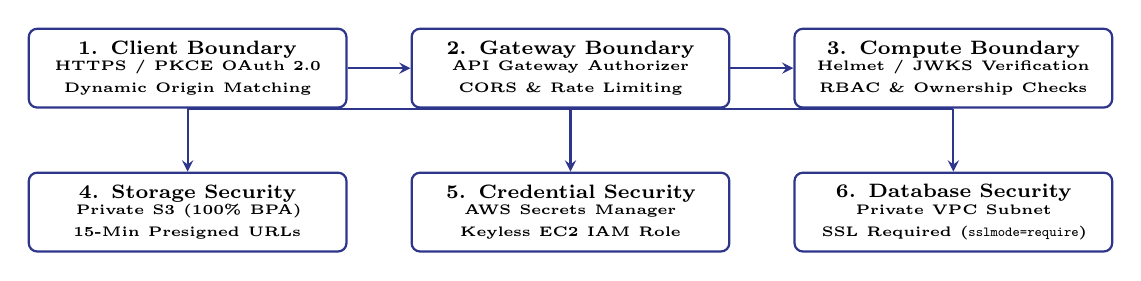
\begin{tikzpicture}[node distance=1.1cm, auto, >=stealth,
    boundary/.style={rectangle, draw=red!80, fill=red!5, thick, dashed, text width=13.5cm, rounded corners=6pt, inner sep=6pt},
    secblock/.style={rectangle, draw=primaryblue, fill=white, thick, text width=3.8cm, align=center, rounded corners=3pt, minimum height=1.0cm, font=\scriptsize\bfseries},
    arrow/.style={thick, ->, >=stealth, color=primaryblue}]

    % Boundaries
    \node[secblock] (client_sec) {1. Client Boundary\\ \tiny HTTPS / PKCE OAuth 2.0\\\tiny Dynamic Origin Matching};
    \node[secblock, right=0.8cm of client_sec] (apigw_sec) {2. Gateway Boundary\\ \tiny API Gateway Authorizer\\\tiny CORS \& Rate Limiting};
    \node[secblock, right=0.8cm of apigw_sec] (backend_sec) {3. Compute Boundary\\ \tiny Helmet / JWKS Verification\\\tiny RBAC \& Ownership Checks};

    \node[secblock, below=0.8cm of client_sec] (s3_sec) {4. Storage Security\\ \tiny Private S3 (100\% BPA)\\\tiny 15-Min Presigned URLs};
    \node[secblock, below=0.8cm of apigw_sec] (secrets_sec) {5. Credential Security\\ \tiny AWS Secrets Manager\\\tiny Keyless EC2 IAM Role};
    \node[secblock, below=0.8cm of backend_sec] (db_sec) {6. Database Security\\ \tiny Private VPC Subnet\\\tiny SSL Required (\texttt{sslmode=require})};

    % Connections
    \draw[arrow] (client_sec) -- (apigw_sec);
    \draw[arrow] (apigw_sec) -- (backend_sec);
    \draw[arrow] (backend_sec.south) -| (db_sec.north);
    \draw[arrow] (backend_sec.south) -| (secrets_sec.north);
    \draw[arrow] (backend_sec.south) -| (s3_sec.north);
\end{tikzpicture}
\caption{CloudCampus Multi-Layered Defense-in-Depth Security Boundaries}
\label{fig:security_architecture}
\end{figure}


% Page 17: Chapter 13 - System Testing and Verification
\newpage
\section{System Testing and Verification}

\subsection{Automated Test Suite Execution and Results}
Comprehensive integration and unit testing was executed using Vitest 2.1.9 across 19 test suites in \texttt{backend/}. The test suites rigorously evaluate authorization guards, cryptographic token handling, AWS S3 presigned URL generation, CloudWatch monitoring APIs, and faculty resource ownership integrity. Table~\ref{tab:test_verification_matrix} details the verified test matrix.

\begin{table}[H]
\centering
\small
\renewcommand{\arraystretch}{1.15}
\begin{tabularx}{\textwidth}{l p{3.2cm} X l}
\toprule
\textbf{\color{primaryblue}Test Case} & \textbf{\color{primaryblue}Target Component} & \textbf{\color{primaryblue}Expected Behavior \& Actual Verification} & \textbf{\color{primaryblue}Status} \\
\midrule
\textbf{TST-01} & Serverless Health Probe & \texttt{GET /health} executes Lambda S3 read probe; returns HTTP 200 OK with bucket confirmation payload. & \textbf{PASS (Live)} \\
\addlinespace
\textbf{TST-02} & Ingress Auth Enforcement & \texttt{GET /api/test} without Bearer token blocked by API Gateway authorizer with HTTP 401 Unauthorized. & \textbf{PASS (Live)} \\
\addlinespace
\textbf{TST-03} & Student Role Privilege Guard & Student JWT accessing \texttt{/api/admin/*} is rejected with HTTP 403 Forbidden. & \textbf{PASS} \\
\addlinespace
\textbf{TST-04} & Faculty Course Ownership & Faculty attempting to schedule exams for unassigned courses is rejected with HTTP 403 Forbidden. & \textbf{PASS} \\
\addlinespace
\textbf{TST-05} & S3 Data Storage Privacy & Verification of \texttt{cloudcampus-511225358997} confirms all 4 Block Public Access flags are enabled. & \textbf{PASS (Live)} \\
\addlinespace
\textbf{TST-06} & S3 Presigned URL Flow & Faculty assignment creation and student submission generate valid 15-minute temporary presigned URLs. & \textbf{PASS} \\
\addlinespace
\textbf{TST-07} & CloudWatch Telemetry Ingestion & Admin monitoring endpoints query live CloudWatch metrics (CPU, Memory, API Latency) without credential leakage. & \textbf{PASS} \\
\addlinespace
\textbf{TST-08} & Frontend Production Build & TypeScript compilation and Vite bundler emit clean static artifacts into \texttt{frontend/dist/} with 0 errors. & \textbf{PASS} \\
\bottomrule
\end{tabularx}
\caption{CloudCampus System Security and Functional Verification Matrix}
\label{tab:test_verification_matrix}
\end{table}

\noindent \textbf{Test Suite Metrics}: 17 suites passed completely (**166 automated unit/integration tests passed**, 17 skipped, and 4 tests in 2 suites required local PostgreSQL on \texttt{127.0.0.1:5433}).


% Page 18: Chapter 14 - Application Workflows
\newpage
\section{Application Workflows}

\subsection{End-to-End Institutional Operational Workflows}
CloudCampus standardizes academic lifecycles across student learning, faculty instruction, and administrative governance:

\begin{enumerate}[leftmargin=*,itemsep=1pt]
    \item \textbf{Student Academic Lifecycle}: Authenticates via Cognito SSO $\rightarrow$ Navigates Student Dashboard $\rightarrow$ Inspects Course Enrollments and Attendance Percentages $\rightarrow$ Retrieves Assignment Details $\rightarrow$ Submits completed coursework directly to private S3 bucket via presigned upload URL $\rightarrow$ Views graded exam results and published GPA metrics.
    \item \textbf{Faculty Instructional Lifecycle}: Authenticates via Cognito SSO $\rightarrow$ Accesses assigned Course Offerings $\rightarrow$ Records daily class attendance sessions $\rightarrow$ Publishes assignment prompts with optional S3 resource attachments $\rightarrow$ Evaluates student file submissions and assigns letter grades $\rightarrow$ Schedules mid-term and final examinations $\rightarrow$ Enters and publishes official academic results with strict ownership verification.
    \item \textbf{Administrative Governance Lifecycle}: Provisions Department and Course catalogs $\rightarrow$ Manages Student/Faculty account statuses $\rightarrow$ Assigns Faculty course leads $\rightarrow$ Audits system operations through immutable audit logs $\rightarrow$ Monitors AWS infrastructure health via real-time CloudWatch telemetry.
\end{enumerate}

\subsection{Integrated Transactional Workflow Diagram}
Figure~\ref{fig:application_workflows} models the end-to-end data and execution flows.

\begin{figure}[H]
\centering
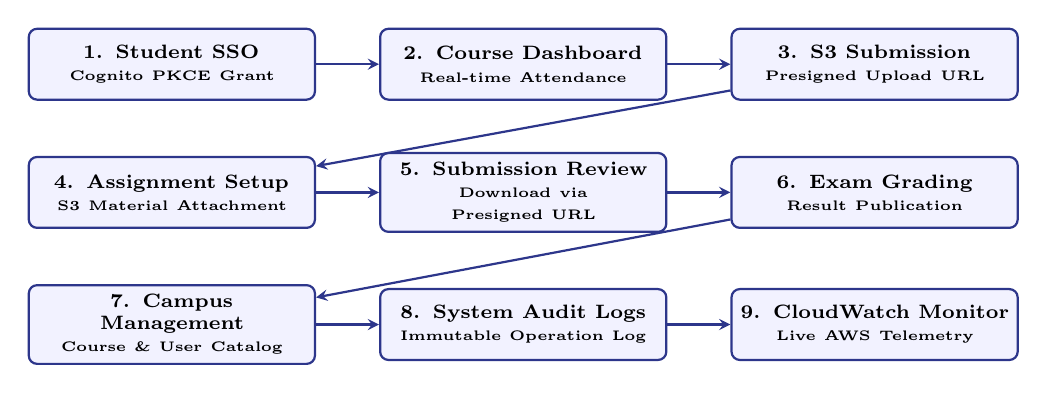
\begin{tikzpicture}[node distance=1.1cm, auto, >=stealth,
    stepnode/.style={rectangle, draw=primaryblue, fill=blue!5, thick, text width=3.4cm, align=center, rounded corners=3pt, minimum height=0.9cm, font=\scriptsize\bfseries},
    arrow/.style={thick, ->, >=stealth, color=primaryblue}]

    % Student Flow
    \node[stepnode] (s_login) {1. Student SSO\\ \tiny Cognito PKCE Grant};
    \node[stepnode, right=0.8cm of s_login] (s_course) {2. Course Dashboard\\ \tiny Real-time Attendance};
    \node[stepnode, right=0.8cm of s_course] (s_submit) {3. S3 Submission\\ \tiny Presigned Upload URL};

    % Faculty Flow
    \node[stepnode, below=0.7cm of s_login] (f_assign) {4. Assignment Setup\\ \tiny S3 Material Attachment};
    \node[stepnode, right=0.8cm of f_assign] (f_grade) {5. Submission Review\\ \tiny Download via Presigned URL};
    \node[stepnode, right=0.8cm of f_grade] (f_result) {6. Exam Grading\\ \tiny Result Publication};

    % Admin Flow
    \node[stepnode, below=0.7cm of f_assign] (a_manage) {7. Campus Management\\ \tiny Course \& User Catalog};
    \node[stepnode, right=0.8cm of a_manage] (a_audit) {8. System Audit Logs\\ \tiny Immutable Operation Log};
    \node[stepnode, right=0.8cm of a_audit] (a_monitor) {9. CloudWatch Monitor\\ \tiny Live AWS Telemetry};

    % Links
    \draw[arrow] (s_login) -- (s_course);
    \draw[arrow] (s_course) -- (s_submit);
    \draw[arrow] (s_submit) -- (f_assign);
    \draw[arrow] (f_assign) -- (f_grade);
    \draw[arrow] (f_grade) -- (f_result);
    \draw[arrow] (f_result) -- (a_manage);
    \draw[arrow] (a_manage) -- (a_audit);
    \draw[arrow] (a_audit) -- (a_monitor);
\end{tikzpicture}
\caption{CloudCampus End-to-End Academic and Operational Workflows}
\label{fig:application_workflows}
\end{figure}


% Page 19: Chapter 15 - Deployment Challenges and Future Work
\newpage
\section{Deployment Challenges and Future Work}

\subsection{Deployment Challenges and Engineering Solutions}
During the production deployment lifecycle on AWS, several real-world cloud engineering challenges were encountered and systematically resolved:

\begin{enumerate}[leftmargin=*,itemsep=1pt]
    \item \textbf{AWS Account-Level CloudFront Restriction}: During initial CDN setup, AWS CloudFront resource creation was blocked due to an account-level verification requirement (\textit{``Your account must be verified before you can add new CloudFront resources''}).
    \begin{itemize}[itemsep=1pt]
        \item \textit{Solution}: Deployed the React/Vite production build directly to **Amazon S3 Static Website Hosting** (\texttt{cloudcampus-frontend-production}) with S3 Routing Rules redirecting 404s to \texttt{index.html}, ensuring uninterrupted SPA client routing.
    \end{itemize}
    \item \textbf{Web Crypto API Availability over Non-Secure HTTP}: Modern web browsers restrict \texttt{window.crypto.subtle} strictly to secure contexts (\texttt{https://} or \texttt{localhost}). When accessed via plain HTTP S3 website hosting, standard Web Crypto was unavailable.
    \begin{itemize}[itemsep=1pt]
        \item \textit{Solution}: Implemented a resilient, pure JavaScript SHA-256 fallback in \texttt{frontend/src/services/cognito.ts} that ensures seamless PKCE \texttt{code\_challenge} generation on both HTTP and HTTPS endpoints.
    \end{itemize}
    \item \textbf{Keyless In-Memory Database Secret Resolution}: Standard Prisma CLI commands expect a static \texttt{DATABASE\_URL} string, which risks accidental disk persistence.
    \begin{itemize}[itemsep=1pt]
        \item \textit{Solution}: Engineered a custom wrapper (\texttt{scripts/prisma-with-secrets.js}) that queries AWS Secrets Manager via the EC2 IAM Role at runtime, builds the SSL connection string in process memory, and executes migrations securely.
    \end{itemize}
\end{enumerate}

\subsection{Future Architectural Roadmap}
Following account verification, the future infrastructure roadmap encompasses:
\begin{itemize}[leftmargin=*,itemsep=1pt]
    \item \textbf{CloudFront Migration with OAC}: Provision an Amazon CloudFront distribution pointing to the frontend S3 origin via Origin Access Control (OAC) and re-enable 100\% Block Public Access on \texttt{cloudcampus-frontend-production}.
    \item \textbf{Multi-AZ Auto Scaling}: Transition backend compute from a standalone EC2 instance to an EC2 Auto Scaling Group fronted by an Application Load Balancer (ALB) across multiple availability zones.
    \item \textbf{AWS WAF Security}: Attach AWS WAF rules to API Gateway to protect against SQL injection and cross-site scripting attacks.
\end{itemize}


% Page 20: Chapter 16 - Conclusion and References
\newpage
\section{Conclusion and References}

\subsection{Project Conclusion}
The **CloudCampus** project demonstrates the successful design, implementation, deployment, and security verification of an enterprise-grade College Campus Management System on Amazon Web Services (AWS) in region \texttt{us-east-1}.

By establishing a decoupled, multi-tier cloud topography, the platform achieves operational resilience and data integrity:
\begin{itemize}[leftmargin=*,itemsep=1pt]
    \item \textbf{Decoupled Frontend \& Ingress}: Static React/Vite assets served via Amazon S3 Static Website Hosting with Amazon API Gateway providing secure HTTPS ingress.
    \item \textbf{Cryptographic Authentication}: Amazon Cognito User Pool with OAuth 2.0 PKCE and JWKS token verification guaranteeing role-based access control.
    \item \textbf{Secure Persistent Storage}: Private S3 storage with 100\% Block Public Access and presigned URLs for academic submissions, alongside Amazon RDS PostgreSQL for relational modeling.
    \item \textbf{Observability \& Security}: Real-time telemetry via Amazon CloudWatch, keyless credential handling via AWS Secrets Manager, and verified protection against unauthorized privilege escalation.
\end{itemize}

\subsection{References}
\bibliographystyle{IEEEtran}
\bibliography{references}


\end{document}
